In this chapter, Redis performance in terms of latency, throughput and system resource requirements is examined. Initially, we will focus on performance under the default configuration of Redis. Subsequently, the scalability characteristics of Redis are explored. Focus is given to the impact of multiple Redis instances running simultaneously on the same machine under various levels of workload.

Unless otherwise stated, all benchmarks are performed to target the required Quality of Service (QoS) of achieving 99th percentile latency under 1 millisecond.


\section{Out of the Box Performance}
\label{sec:redis-default}
Firstly, in order to understand the baseline performance of Redis we consider the default configuration of Redis. A Redis deployment can be started with the following command:
\begin{lstlisting}
redis redis.conf --port 11120
\end{lstlisting}

By default, a Redis deployment comes with a default configuration file \texttt{redis.conf}\cite{RedisConfiguration}. Any options specified in the configuration file can be overridden from the command line by prefixing them with \texttt{--}, in our case we are overriding the port number and setting it to 11120. All other configuration options remain unmodified.

In order to understand the default Redis performance, we design the benchmark to exert an increasing level of load on the Redis server. Initially, we start with 2 threads and 1 connection per each thread on all workload generating clients, there are 7 such clients in our setup.  In our workload, we define the key space to be up to 100 million keys with an object size of 64 bytes yielding around 6.4 GB of data while the memory capacity of the server is 8GB and therefore data should not be swapped out of main memory. The workload generating clients are executed with the following command:

\begin{lstlisting}
memtier -s nsl200 -p 11120
    -c <connection_count> -t 2
    -P redis
    --random-data --data-size=64
    --key-minimum=1 --key-maximum=100000000
    --test-time=400
\end{lstlisting}

The number of connections per each thread is increased linearly in each subsequent benchmark run. Each workload is executed over the course of 400 seconds and the data is randomly generated with keys drawn from a uniform distribution between 1 and 100 million.


\subsection{Latency vs Throughput}

\begin{figure}[h]
    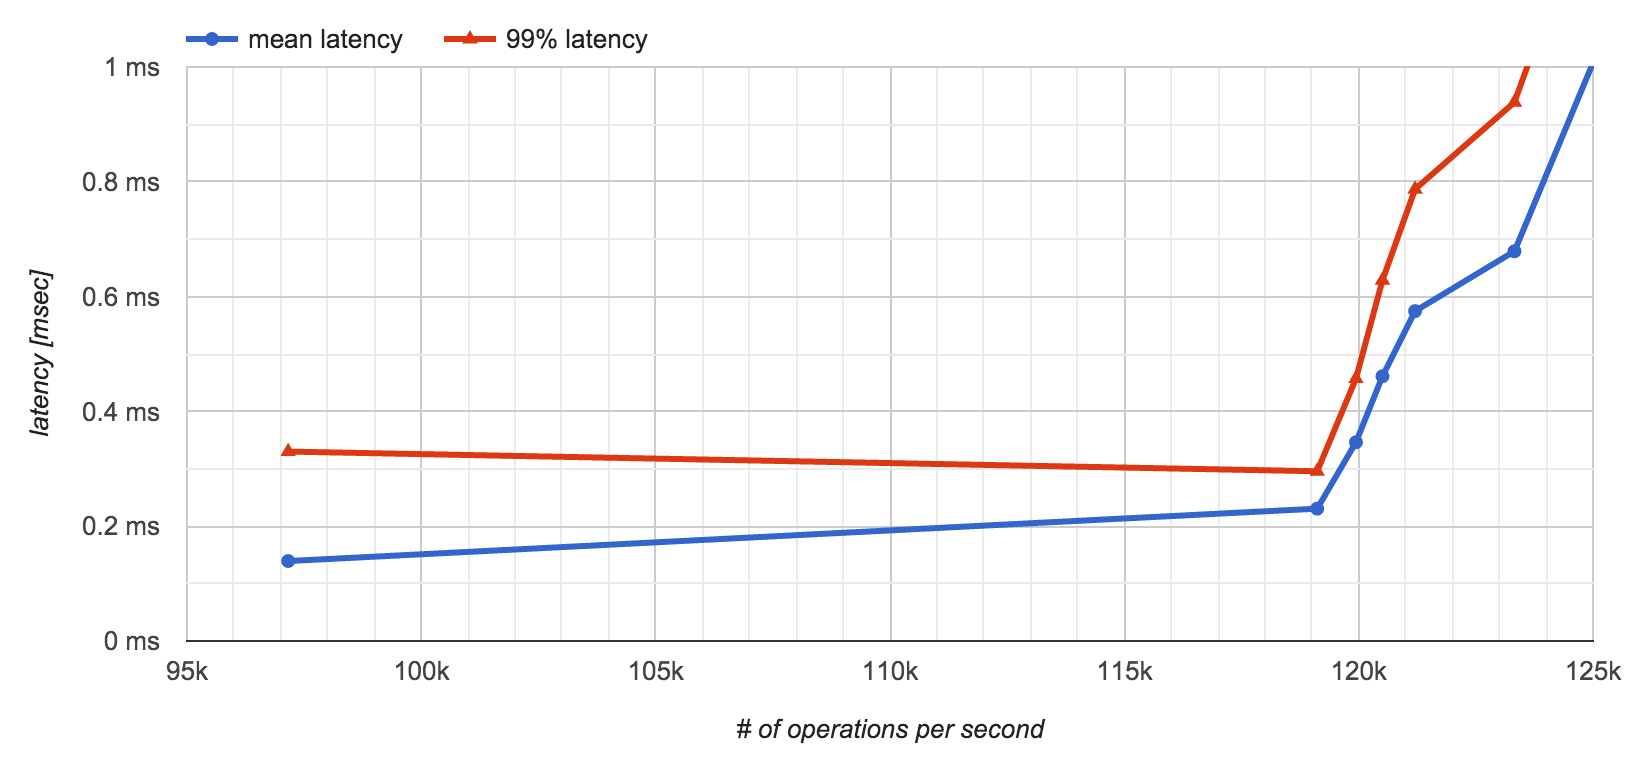
\includegraphics[width=\textwidth]{./res/6_default_latency_ops.png}
    \caption{Redis: Throughput vs Mean and 99th percentile latency}
    \label{fig:redis-default-latency-ops}
\end{figure}

Figure \ref{fig:redis-default-latency-ops} plots the relationship between mean latency and the 99th percentile latency on the vertical axis and the number of operations per second on the horizontal axis. The graph has been trimmed to show only data which satisfies the QoS requirements.

We can observe that the number of operations Redis processes increases steadily until it reaches 119k requests per second at which point a further increase in throughput comes at a disproportionately grater cost in both mean and 99th percentile latency. The peak throughput observed under the QoS requirements is around 123k requests per second.

The performance degrades significantly with an increased workload beyond the peak shown at 123k requests per second. The throughput remains the same while the mean and the 99th percentile latency spikes heavily.


\subsection{CPU Utilization}

\begin{figure}[h]
    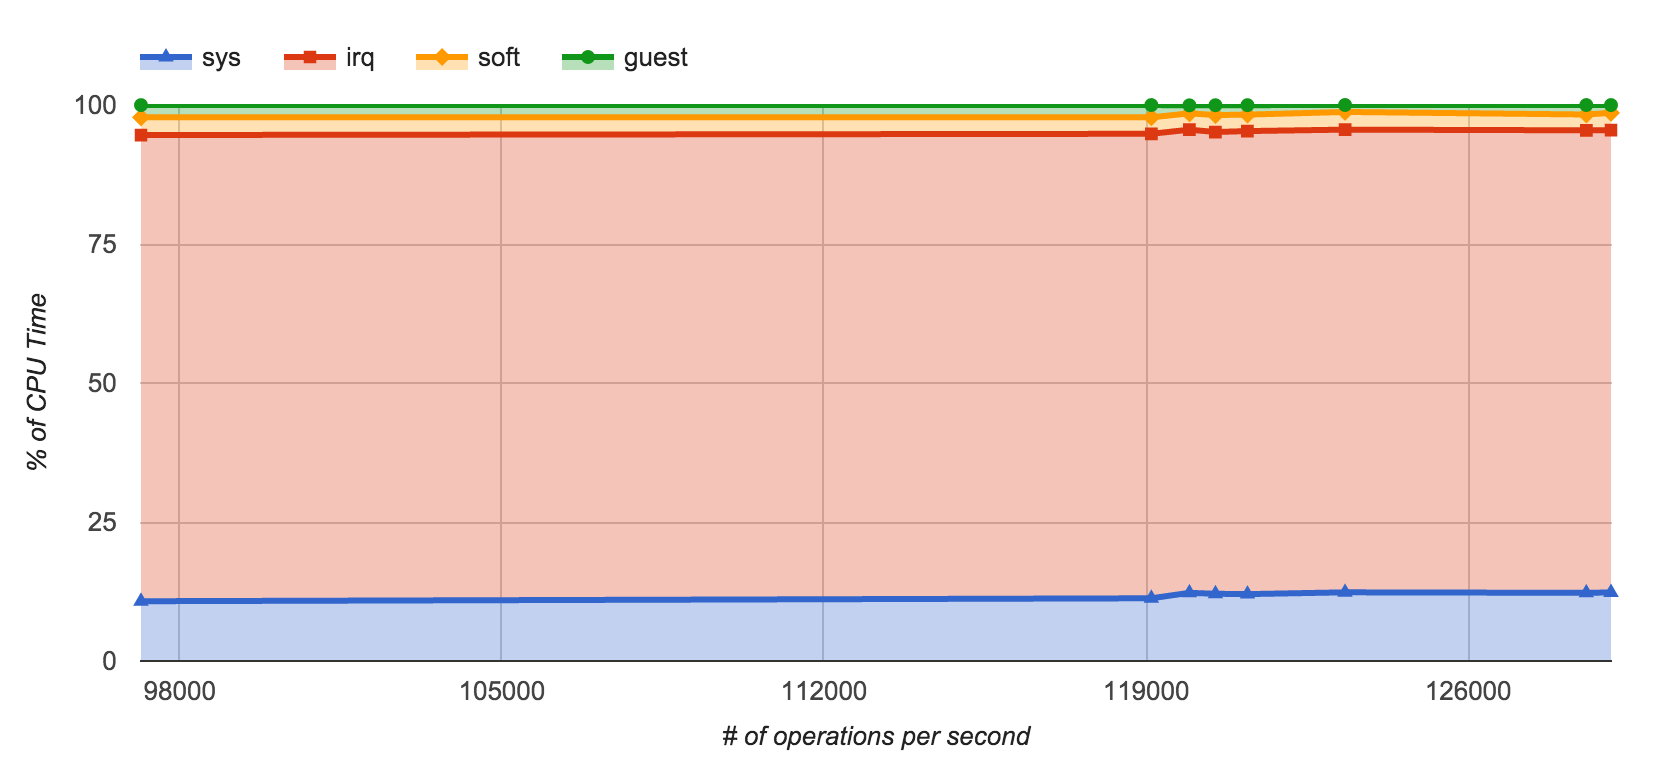
\includegraphics[width=\textwidth]{./res/6_default_cpu.png}
    \caption{Redis: CPU Utilization}
    \label{fig:redis-default-cpu}
\end{figure}

Figure \ref{fig:redis-default-cpu} outlines the CPU utilization in terms of time spent processing system calls (sys), servicing hardware interrupts (irq), handling software interrupts (soft) and processing related to Redis (guest).

We can observe that servicing hardware interrupts consumes the majority of the processing time - 83 percent. This is the result of receiving and dispatching a large number of requests through the NIC. The amount of CPU time devoted to processing system calls is about 10 percent while processing software interrupts accounts for 3 percent. Redis itself requires only about 2 percent of the overall CPU time.

Redis appears to be network constrained rather than CPU constrained in the workload examined above. This is reasonable as Redis is executing within one main event loop therefore it does not require locking and does not generate heavy load on the CPU when looking values up in the cache.


\section{Multiple Redis Instances}
\label{sec:multiple-redis-instances}

As seen in section \ref{sec:redis-default}, Redis cannot increase overall throughput of the system with only a single instance as only a single core is capable of processing requests and becomes the bottleneck. An immediate solution to this problem is to provision a larger number of instances on a multi-core system in order to better utilize the hardware resources.

In this benchmark, we examine the effects increased number of Redis instances with respect to latency, 99th percentile latency and overall throughput of the system. Additionally, we examine the effect of multiple instances on the CPU usage.

Firstly, multiple instances of Redis can be spawned easily on the server by binding them to distinct port numbers. Out of the box, Redis does not provide the capability to proxy multiple instances of Redis through a single port in order to load balance the instances. There is the option to configure a Redis cluster, however, the intended use case is primarily for resiliency and fail over. In this benchmark, we consider a simpler scenario where each instance is isolated from each other and acts as an independent cache. This is a simplification of a real world scenario, however, a large deployment of Redis could be designed to partition the key space and utilize multiple independent instances similarly. The Redis application can be spawned with the following script:

\begin{lstlisting}
for i in [1..n]
    redis-server redis.conf --port (11120 + i) --maxmemory (6 / i)gb
\end{lstlisting}

Note that we are explicitly specifying the maximum amount of memory each instance will be allocated. In our case, we partition 6 GB of memory space evenly between the individual instances.

Secondly, in order to obtain comparable results, the load exerted on the Redis cache must remain constant. The load itself, however, needs to be partitioned across all of the instances of Redis evenly. In order to achieve this, each workload generating client spawns \texttt{i} instances of the benchmark and targets its respective Redis instance. We use the following script to start the workload generating clients:

\begin{lstlisting}
for i in [1..n]
    memtier -s nsl200 -p <port>
        -c round(16 / i)
        -t 1
        -P redis
        --random-data --data-size=64
        --key-minimum=1 --key-maximum=round(100000000 / i)
        --test-time=400
\end{lstlisting}

Initially, we start with 16 connections and 1 thread. As we increase the number of instances, the number of connections goes down, however, a larger number of instances are deployed. Note that we are using a \texttt{round} function to ensure that the number of connections as well as the maximum key are integers. In order to smooth out load variance caused by integer divisibility, we consider two cases. One in which the \texttt{round} function is defined as the \texttt{ceiling} function and the other when it is defined as the \texttt{floor} function. The results of both types of the \texttt{round} function are then averaged. If a higher number of workload generating clients were available for the experimentation, the round approach would not be required.

Furthermore, the generated dataset is 6.4GB (100 million keys * 64 bytes of data). This is by design and leads to evictions in the cache as the size approaches the maximum.


\subsection{Latency and Throughput}

\begin{figure}[h]
    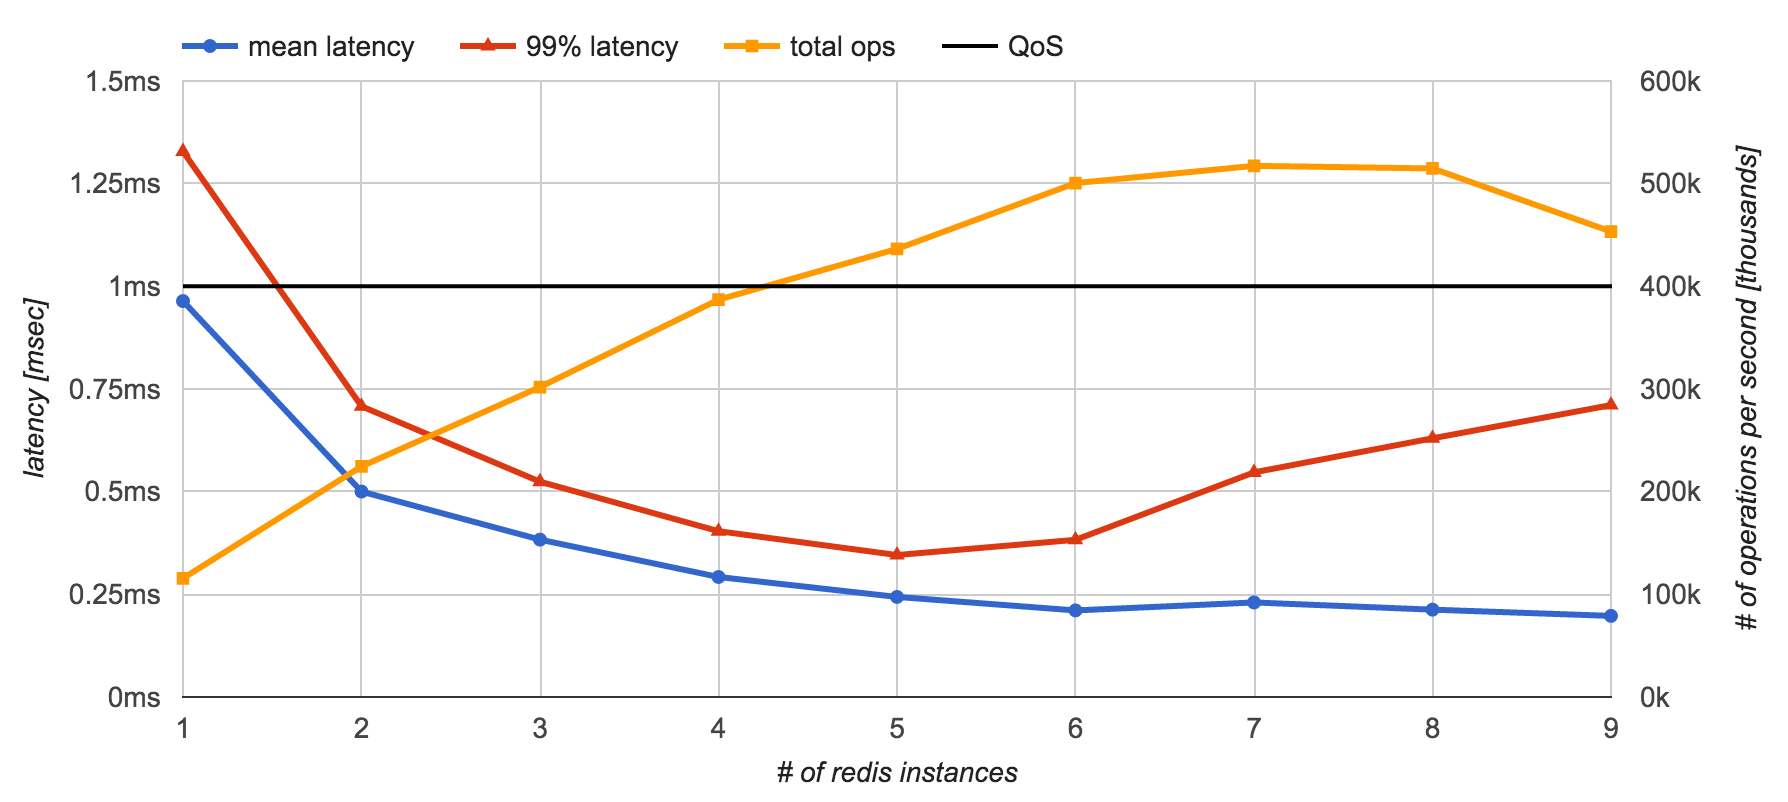
\includegraphics[width=\textwidth]{./res/6_instances_latency_ops.png}
    \caption{Redis Instances: Latency, Throughput vs Number of instances}
    \label{fig:redis-instances-latency-ops}
\end{figure}

Figure \ref{fig:redis-instances-latency-ops} plots the relationship between the number of Redis instances running simultaneously on the cache server against the mean and 99th percentile latency on the left vertical axis and the total number of operations per second on the right axis. The black line positioned at 1 ms outlines the QoS target of the benchmark.

The mean latency (blue) decreases steadily as the number of Redis instances increases. At five Redis instances, the mean latency flattens out and remains stable as the number of instances is increased further.

The 99th percentile latency (red), on the other hand, experiences a sharp decrease as the number of instances is increased from 1 to 2 which brings the 99th percentile latency within the desired QoS constraints. As the number of instances increases further, the 99th percentile latency continues to decrease steadily. The minimum is reached at 5 instances with latency of 0.346 ms. A further increase in the number of instances results in higher 99th percentile latency.

The total number of operations increases steadily as the number of instances increases, peaking at 517,000 requests per second with 7 and 8 instances. A further increase in the number of instances results in a decrease in the total number of operations.

The QoS target is achieved in all but the 1 instance scenario. This is due to significantly larger load exerted on a single instance which in the subsequent multi-instance benchmarks gets distributed across the larger number of instances and therefore satisfies the QoS constraints.

Additionally, Redis manages to scale quite well as the number of instances increases up to 6. At this point, there are as many instances as there are CPU cores on the Redis server. Consequently, at 6 instances we achieve near minimum 99th percentile latency while also achieving near maximum throughput.

Furthermore, at 6 instances the 99th percentile latency is at around one third of the accepted QoS constraint. In real world deployment, it should be possible to utilize this gap to increase the throughput further. In our benchmarks, we have not been able to exert a load which would both increase throughput as well as increase the 99th percentile underutilization. This is due to a limited number of client benchmarking hosts to effectively tune the load to the required level.


\subsection{CPU Utilization}

\begin{figure}[h]
    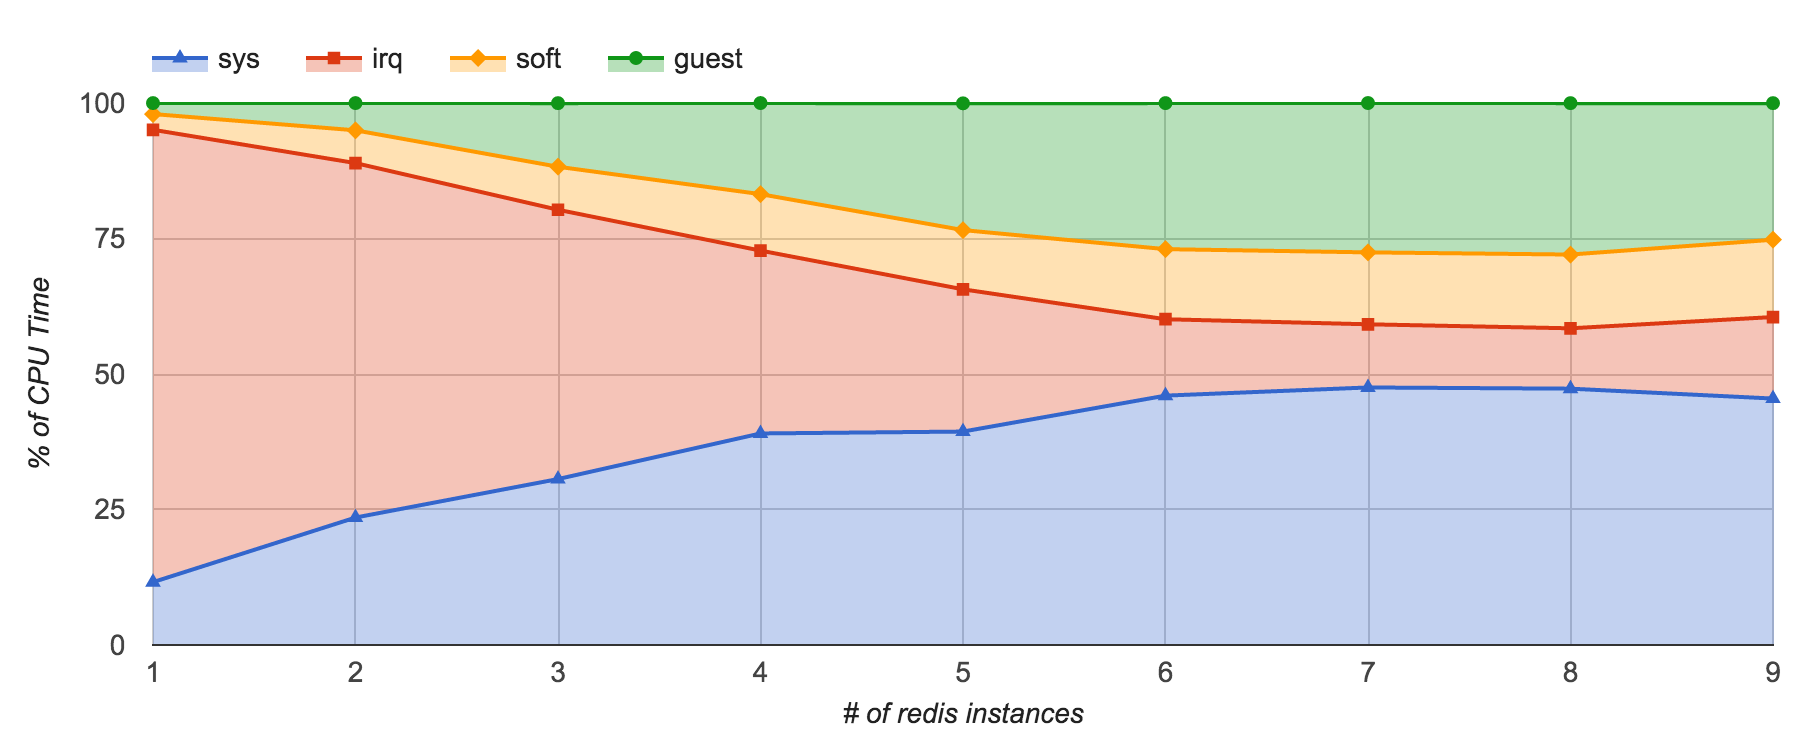
\includegraphics[width=\textwidth]{./res/6_instances_cpu.png}
    \caption{Redis Instances: CPU Utilization vs Number of Instances}
    \label{fig:6_instances_cpu.png}
\end{figure}

Figure \ref{fig:6_instances_cpu.png} presents the relationship between the number of instances and the CPU utilization.

Firstly, the CPU usage of Redis (green), \textit{guest}, increases as the number of instances provisioned increases steadily. At 6 instances and more, the overall CPU usage remains fairly constant accounting for 27 percent of the total CPU utilization. This is due to the server having 6 CPU cores, requiring context switching between applications rather than parallel processing.

Secondly, the CPU dedicated to software interrupts (yellow), \textit{soft}, follows a similar pattern to Redis. As the number of instances increases, so does the CPU usage dedicated to software interrupts. At 6 instances or more, the CPU utilization remains stable, accounting for 10 percent of the total usage. Software interrupts are inherently correlated to the software applications running on the server and therefore it is reasonable to observe a similar pattern between software interrupts and the application itself.

Thirdly, the CPU usage required by the operating system (blue), \textit{sys}, grows steadily as the number of Redis instances increases. At 6 instances or more, the operating system CPU usage peaks and remains stable at 48 percent.

Finally, the portion of the CPU time dedicated to processing hardware interrupts (red), \textit{irq}, decreases steadily as the number of Redis instances increases. This is due to batching of requests at the network interface card. At 6 or more instances, hardware interrupt servicing takes up about 11 percent of the total CPU usage.

Despite the increased resource requirements by Redis, it still only accounts for about 27 percent CPU usage at 6 processes with majority of the CPU time spent in the operating system and or networking. The observation from the single instance benchmark in the previous section therefore extends to a multi instance setup. Redis appears to be network intensive rather than CPU intensive.


By spawning multiple instances of Redis, we have been able to significantly increase the overall performance of the server cache. Running multiple simultaneous instances, however, requires the key space to be partitioned.


\section{Pinned Redis Instances}

In the previous section we have observed that the performance of a Redis server can be greatly improved by provisioning multiple Redis instances simultaneously. Pinning processes to distinct cores is suggested to improve tail latency \cite{leverich2014reconciling}. In this section, we examine the effect process pinning has on the performance of Redis. We consider exactly the same workload as in the previous section \ref{sec:multiple-redis-instances} as well as exactly the same server setup with the exception of pinning the Redis processes. That is, the workload is kept constant while it is partitioned across multiple instances.

A Redis process can be pinned to a unique core through the use of the \texttt{taskset} utility as follows:

\begin{lstlisting}
taskset -pc <redis_pid> <core_id>
\end{lstlisting}

The Redis processes identified as \texttt{redis pid} is pinned to the CPU core identified by \texttt{core id}. We can identify the process id of a Redis application through the \texttt{ps} command. When running more Redis applications than there are CPUs, we assign it to the \textit{n}th index of the application modulo the total number of cores, which is 6.


\subsection{Pinned Latency and Throughput}

\begin{figure}[h]
    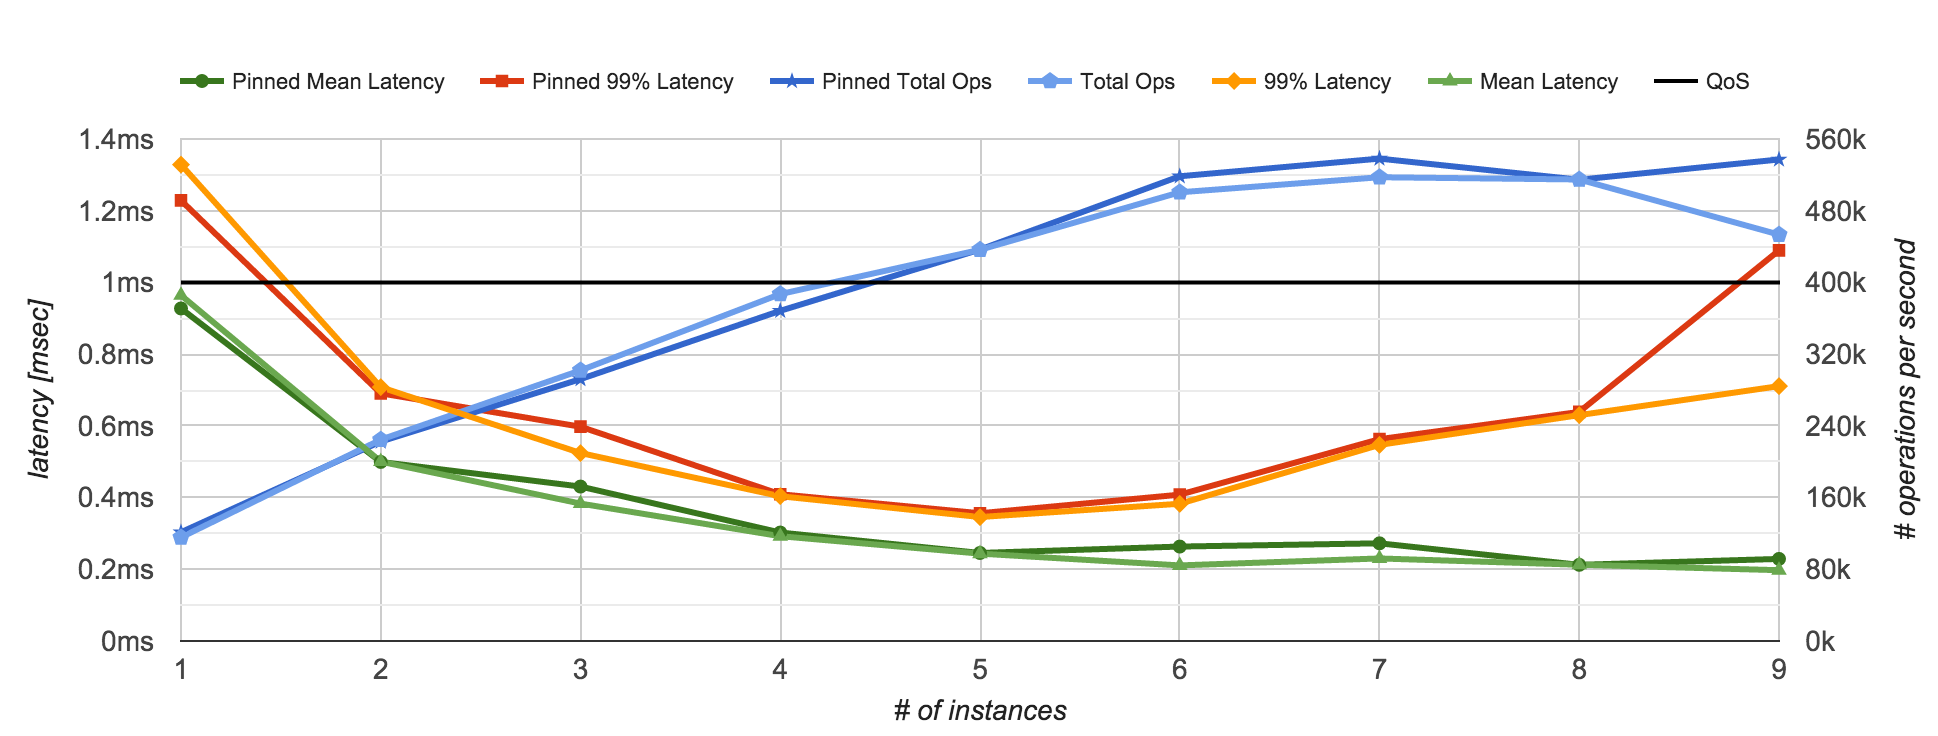
\includegraphics[width=\textwidth]{./res/6_pinned.png}
    \caption{Redis Instance Pinning: Instances vs Latency and Throughput}
    \label{fig:6_pinned.png}
\end{figure}

Figure \ref{fig:6_pinned.png} plots the relationship between the number of instances on the horizontal axis, latency on the left vertical and throughput on the right vertical. Additionally, the performance obtained without pinning are plotted alongside the pinned results.

We can observe that pinning  Redis processes results which strongly correlate to the results of the unpinned benchmark. Across mean latency, 99th percentile latency and throughput, there is very little variance in the performance observed.


\subsection{Redis Persistence}
TODO


\section{Object Size}
In this section, the impact of the size of the object stored in the cache is investigated. Redis imposes no restrictions on the size of objects stored in the cache.

In order to investigate the impact of object size on the cache, we consider a benchmark with an increasing object size. The object size is increased in powers of two starting at 2 bytes and ranging to 512 KB. This allows us to capture the majority of important sizes commonly used when designing applications.

The server configuration remains the same as the current best found configuration, the multi-instance configuration with 6 instances. The clients are configured as follows:

\begin{lstlisting}
for i in [1..19]
    memtier -s nsl200 -p <port>
        -c 3
        -t 1
        -P redis
        --random-data --data-size=pow(2, i)
        --key-minimum=1 --key-maximum=(1066666666 / pow(2, i))
        --test-time=400
\end{lstlisting}

We run 19 iterations of the benchmark since 512 KB is equivalent to 2 to the power of 19 bytes. The \texttt{data-size} is configured to be increasing in powers of 2. The key range is defined as 6.4 GB split across 6 instances and further accounts for the increased size. Therefore, we arrive at \texttt{6.4 GB / (6 * data-size)} which is equivalent to \texttt{(1066666666 / pow(2, i))}.


\subsection{Latency and Throughput}

\begin{figure}[h]
    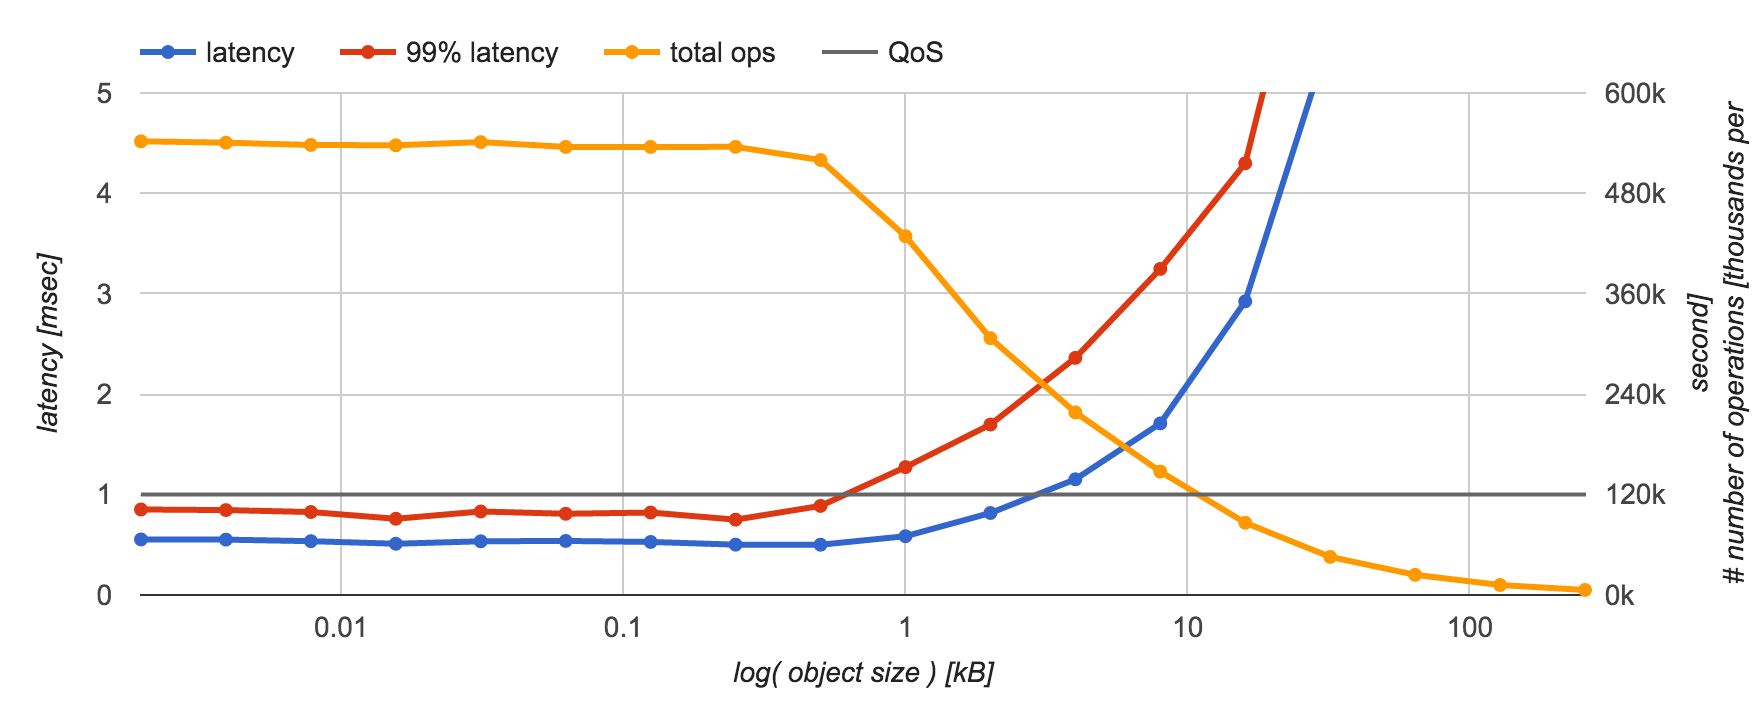
\includegraphics[width=\textwidth]{./res/6_object_size_latency_ops.png}
    \caption{Redis Object Size: Latency and Throughput}
    \label{fig:6_object_size_latency_ops.png}
\end{figure}

Figure \ref{fig:6_object_size_latency_ops.png} displays the relationship between object size on the horizontal logarithmic axis, latency on the left vertical axis and throughput on the right vertical axis.

Firstly, as object size increases up to 512 bytes, the mean latency remains stable at 0.55 ms. Beyond 512 bytes, the mean latency starts to increase and climbs beyond the desired QoS constraint at object size of 4 KB. A further increase in object size leads an disproportionately greater increase in mean latency.

Secondly, the 99th percentile follows the same pattern as the mean latency, however, it begins to climb over the desired QoS sooner, at object size of 1 KB.

Thirdly, the number of operations per second remains constant for object sizes under 256 bytes. An increase in object size decreases the number of operations per second. This is a reasonable result as an increase in the object size leads to higher bandwidth requirements and therefore leads to a lower number of operations per second.

Overall, Redis appears to be capable to scale well with object sizes up to 512 bytes. Larger object sizes put additional strain on the cache and require buffering which leads to increased latency of the average, and therefore 99th percentile, request. Primarily, Redis is not designed to store large (1KB+) values. It is, however, possible to partition large values into smaller ones and perform assembly/disassembly of the value on the client side.

\subsection{CPU Utilization}
\begin{figure}[h]
    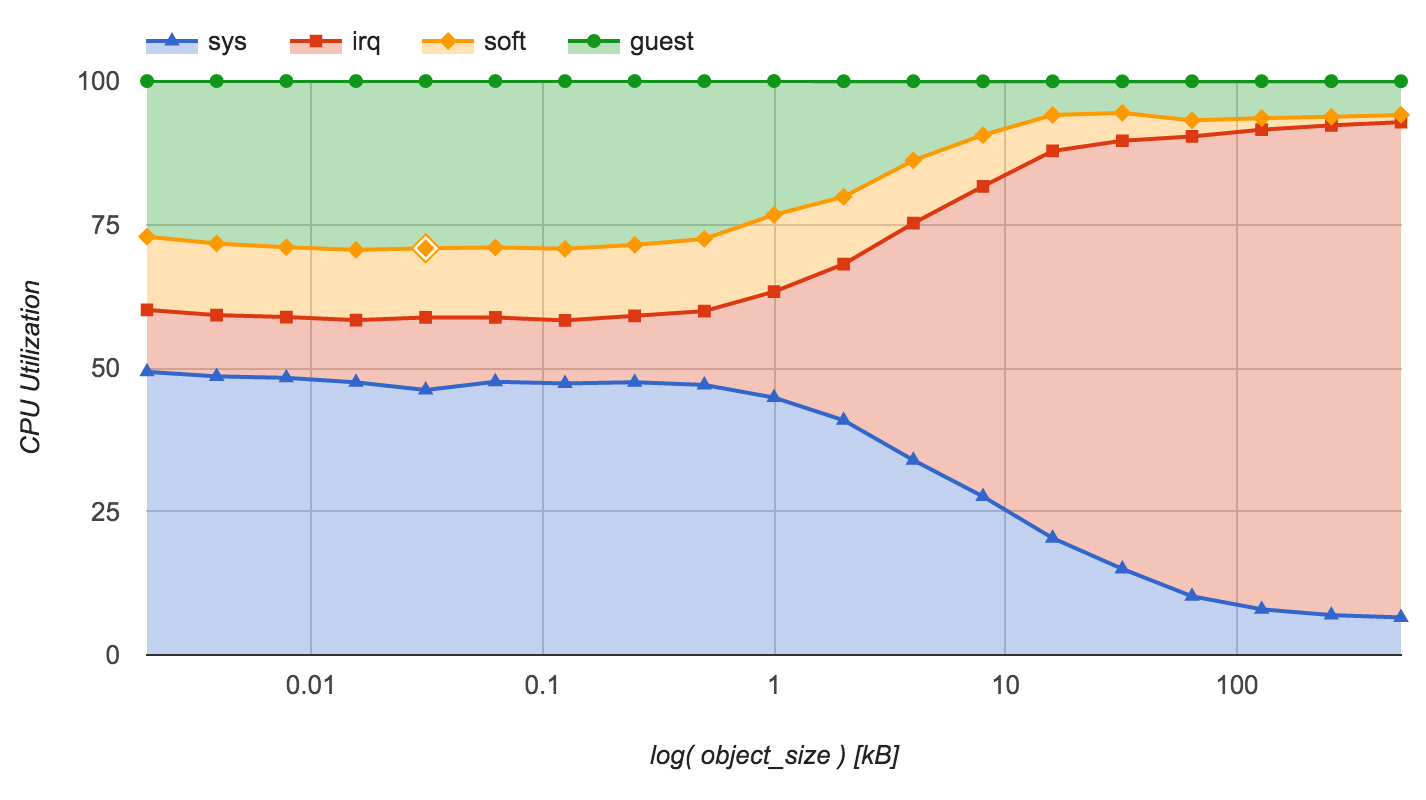
\includegraphics[width=\textwidth]{./res/6_object_size_cpu.png}
    \caption{Redis Object Size: CPU Usage}
    \label{fig:6_object_size_cpu.png}
\end{figure}

Figure \ref{fig:6_object_size_cpu.png} displays the relationship between object size and CPU usage on the Redis server.

Firstly, as object size increases up to 1 KB, the operating system (sys) requires about 47 percent of the total time to process the incoming requests and dispatch them to the relevant applications. As object size increases further, the time required decreases as the number of operations decreases.

Secondly, the Redis applications (guest) require 27 percent of the total time when processing requests under 1 KB, with requests larger the direct cost of running Redis decreases as there are less requests to process. A similar pattern holds for the software interrupts (soft), as there are less requests coming.

Finally, the time allocated to servicing hardware interrupts (irq) remains at 12 percent below 1KB, with object size increases beyond 1 KB, there is significant increase in the time required to service hardware interrupts. This is due to buffering of large objects and is effectively the cause of high mean and 99th percentile latency as well as low throughput.


Overall, Redis is designed to work well with objects sizes below 1 KB. As the object size increases, the cache experiences a degraded performance due to network buffering.

\section{Key Distributions}
TODO

\subsection{Gaussian distribution}
TODO

\subsection{Zipf distribution}
TODO